\documentclass[12pt,a4paper]{article}
\usepackage[a4paper,top=1.5cm, bottom=1.5cm, left=1.5cm, right=1.5cm]{geometry}
\usepackage[T2A]{fontenc}
\usepackage[utf8]{inputenc}
\usepackage[russian]{babel}
\usepackage{amsmath}
\usepackage{amssymb}
\usepackage{graphicx}
\usepackage{floatrow}
\usepackage{booktabs}
\usepackage{wrapfig}
\usepackage{indentfirst}
\usepackage{lipsum}
\usepackage{subcaption}
\usepackage{float}
\usepackage{enumitem}
\restylefloat{table}

\newcommand{\figref}[1]{(см. рис. \ref{#1})}
\newcommand{\e}[1]{\text{$\cdot10^{#1}$}}

\title{Лабораторная работа 5.2.1 \\ Опыт Франка-Герца}
\author{Симанкович Александр\\ Б01-108}
\date{02.12.2023}

\begin{document}
	\maketitle
	
	\section*{Аннотация}
	
	В работе экспериментально подтверждается воспроизводимость результатов опыта Франка-Герца.
	Для опыта используется лампа ЛМ-2 (наполнение: гелий, $\sim 1$ Торр). Определяется энергия перехода между основным и первым возбужденным состоянием атома гелия: $\Delta V = (19.3 \pm 0.4)$ В. 

	\section*{Описание опыта}
	
	\begin{wrapfigure}[12]{r}{6.0cm}
		%              ^^ number of occupied rows
		\includegraphics[width=\linewidth]{res/simple_scheme.png}
		\caption{Принципиальная схема опыта.}
		\label{fig:simple_scheme}
		\vspace{0pt}
	\end{wrapfigure}
	
	Опыт Франка-Герца является одним из простейших опытов, подтверждающих существование дискретных уровней энергии атомов.
	
	В опыте используется трехэлектродная лампа, наполненная разреженным одноатомным газом. Катод испускает электроны, разгоняемые полем между катодом и сетчатым анодом. Между анодом и коллектором электроны летят под действием запирающего электрического поля.
	
	Если энергия электронов недостаточно высока для возбуждения или ионизации атомов газа, то возможны только упругие соударения, в результате которых электроны почти не теряют энергию. При повышении разгоняющего напряжения все больше электронов долетает до коллектора. При достижении энергии возбуждения и ионизации атомов, электроны начинают терять энергию в неупругих столкновениях. После столкновения энергии электрона может не хватить, чтобы преодолеть запирающее поле, из-за чего он не долетает до коллектора. Ток падает.
	\begin{wrapfigure}[12]{r}{5.0cm}
		%              ^^ number of occupied rows
		\includegraphics[width=\linewidth]{res/iv.png}
		\caption{Зависимость тока от напряжения катод-анод.}
		\label{fig:iv}
		\vspace{0pt}
	\end{wrapfigure}
	
	Дальнейшее повышение напряжения увеличивает ток, поскольку электроны, испытавшие неупругое соударение, успевают набрать достаточную энергию, чтобы долететь до коллектора. Однако, при достижении энергии, достаточной для двух неупругих столкновений, ток вновь падает. Таким образом, на графике наблюдаются падения тока через равные промежутки напряжений, соответствующие энергии возбуждения атомов газа.
	
	\newpage
	\section*{Методика эксперимента}
	
	\begin{figure}[H]
		\centering
		\includegraphics[width=0.9\linewidth]{res/block_scheme.png}
		\caption{Схема установки.}
		\label{fig:block_scheme}
	\end{figure}
	
	\begin{figure}[H]
		\centering
		\begin{minipage}{0.75\textwidth}
			\centering
			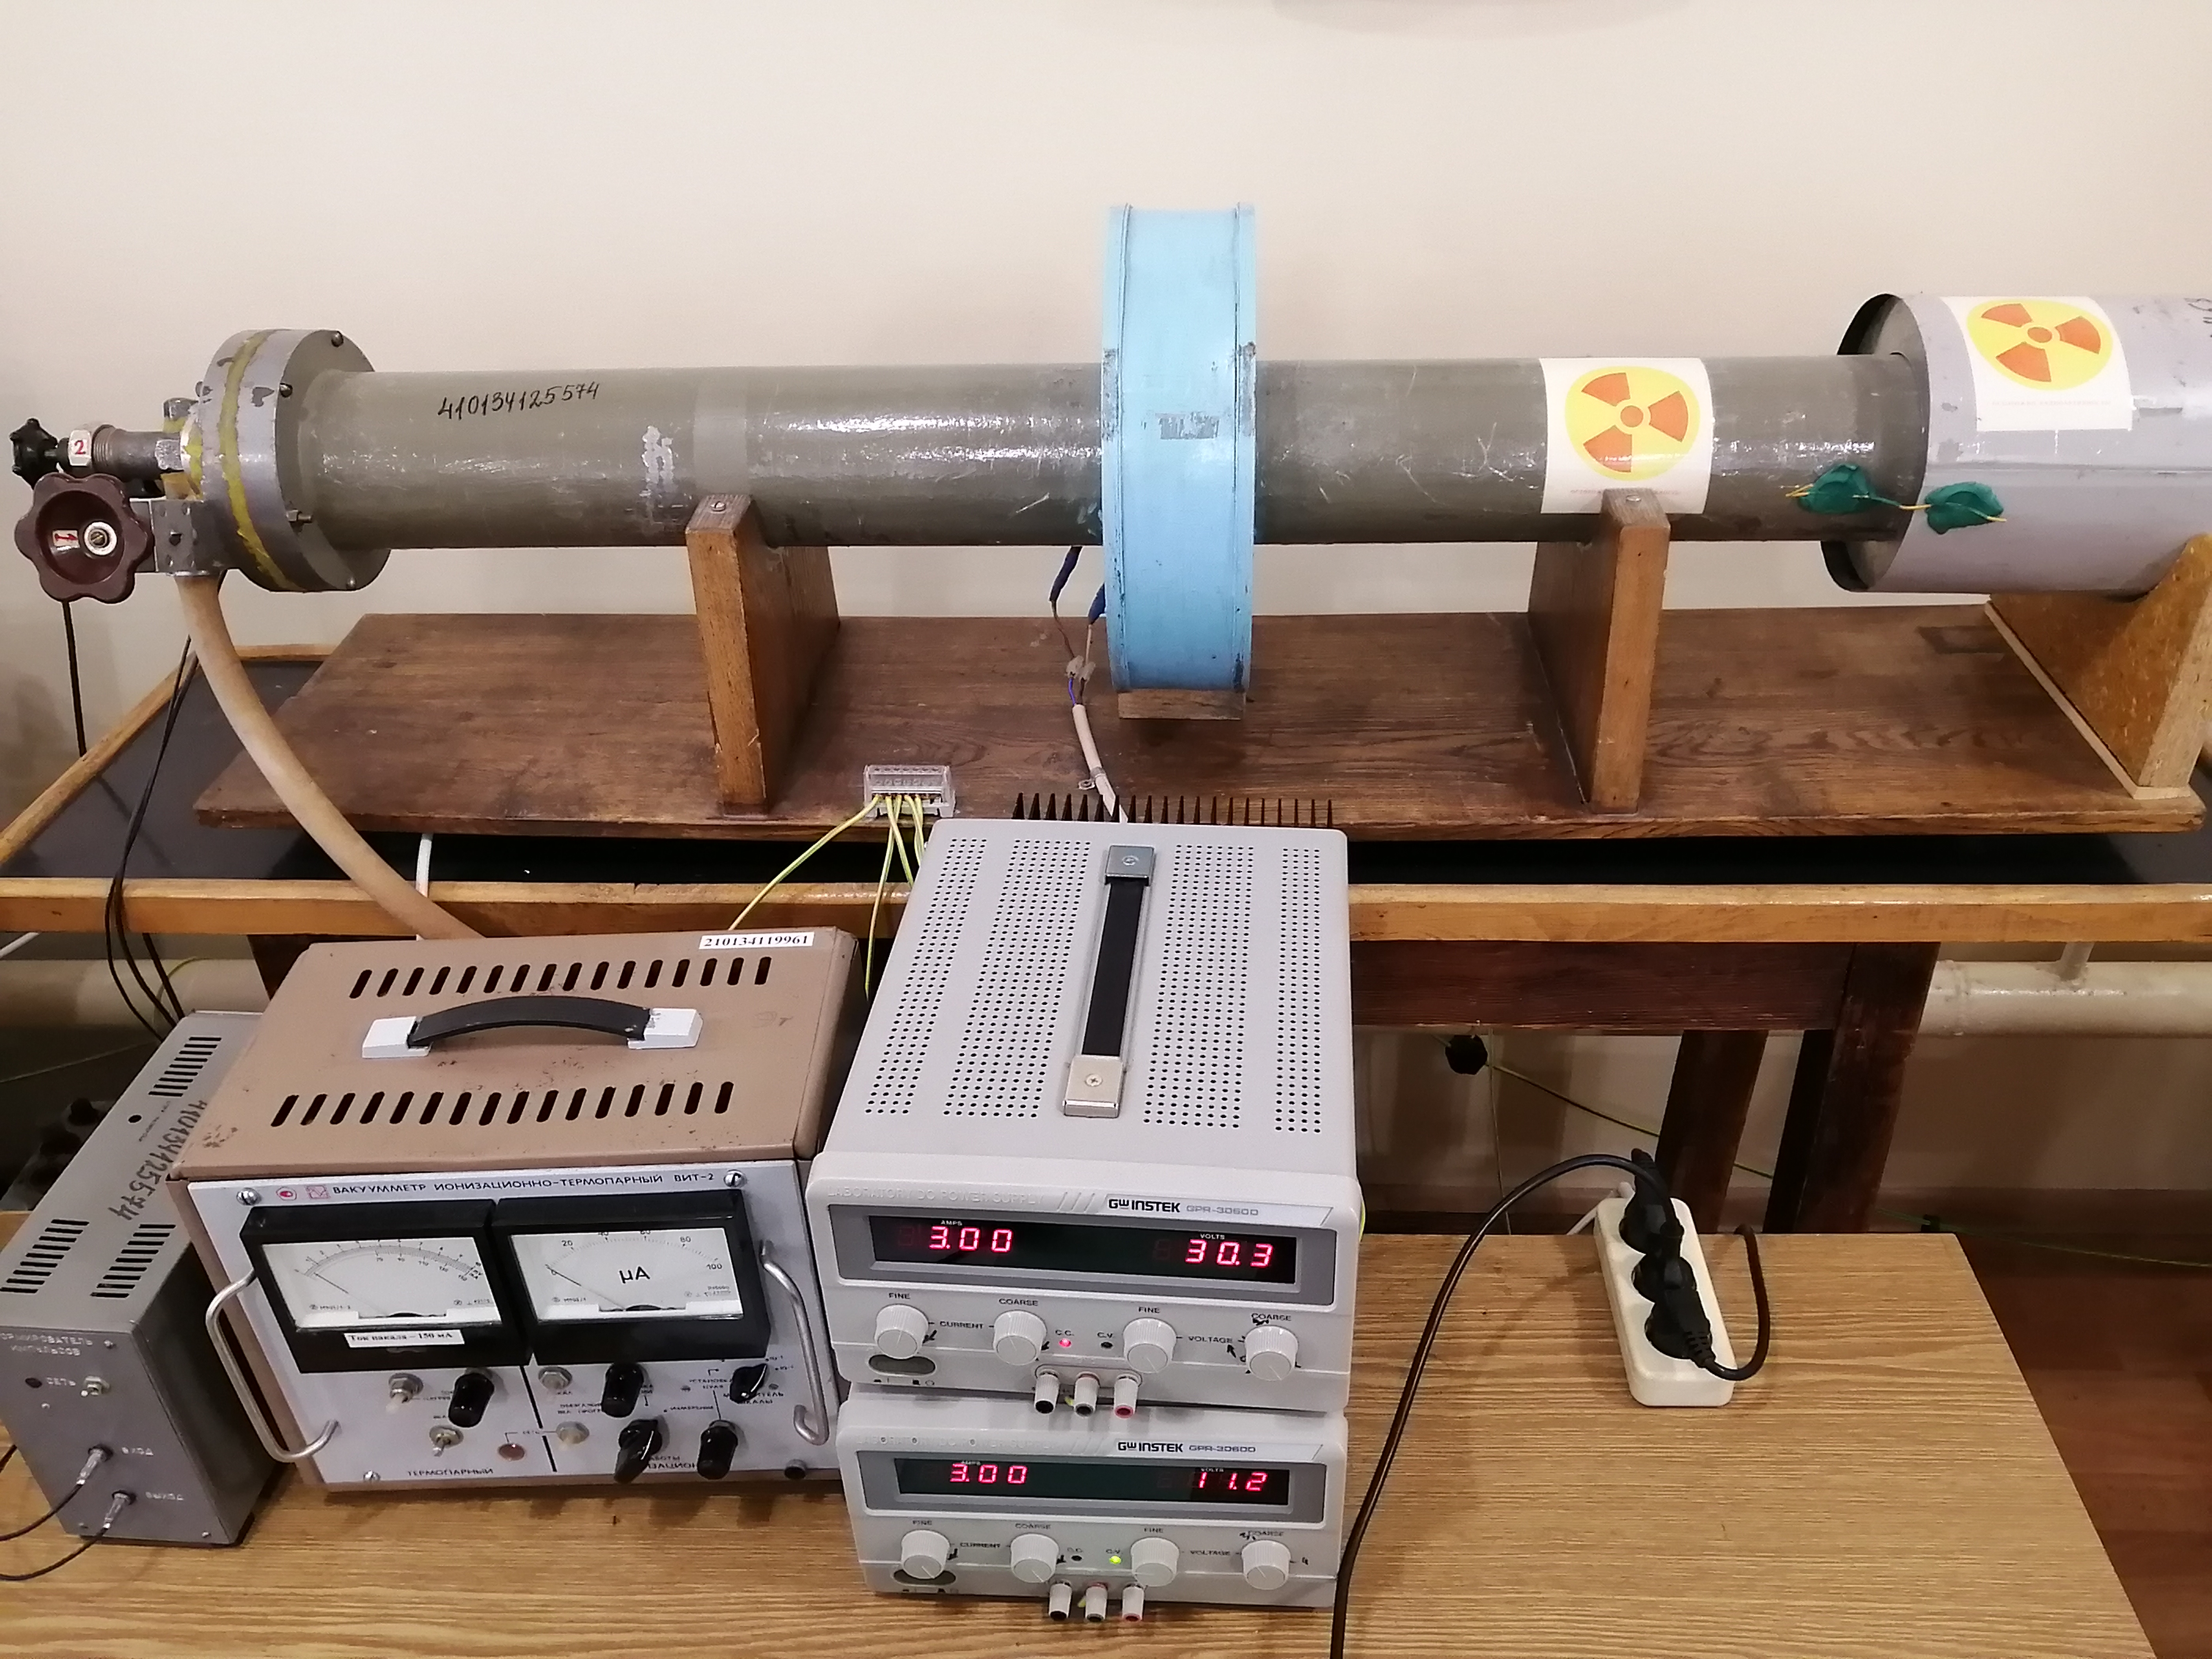
\includegraphics[width=0.9\linewidth]{photos/setup.jpg}
		\end{minipage}%
		\begin{minipage}{0.24\textwidth}
			\centering
			\includegraphics[width=0.9\linewidth]{photos/lamp.jpg}
		\end{minipage}
		\caption{Фотография установки..}
		\label{fig:setup}
	\end{figure}

	В опыте используется лампа ЛМ-2, заполненная гелием до давления $\sim 1$ Торр. Электроны испускаются вольфрамовым катодом, который нагревается от источника С. Лампа состоит из осевого катода, пары коаксиальных ему спиралей в качестве анода и коаксиального полого цилиндра-коллектора.
		
	В первой части работы измерения проводятся с помощью осциллографа. На графиках наблюдается зависимость напряжения коллектора $V_{\text{коллектор}}$ от напряжения катод-сетка $V_{\text{катод}}$.
	
	Во второй части работы измерения проводятся статически, с помощью вольтметров. Данные измерения повышают точность эксперимента, избавляя от инерционных эффектов, которые возникают при использовании осциллографа.

	\newpage

	\section*{Результаты}
	
	\subsection*{Динамика}
	
	В соответствии с вышеописанной методикой получаем осциллограммы ВАХ лампы.

	\begin{figure}[H]
		\centering
		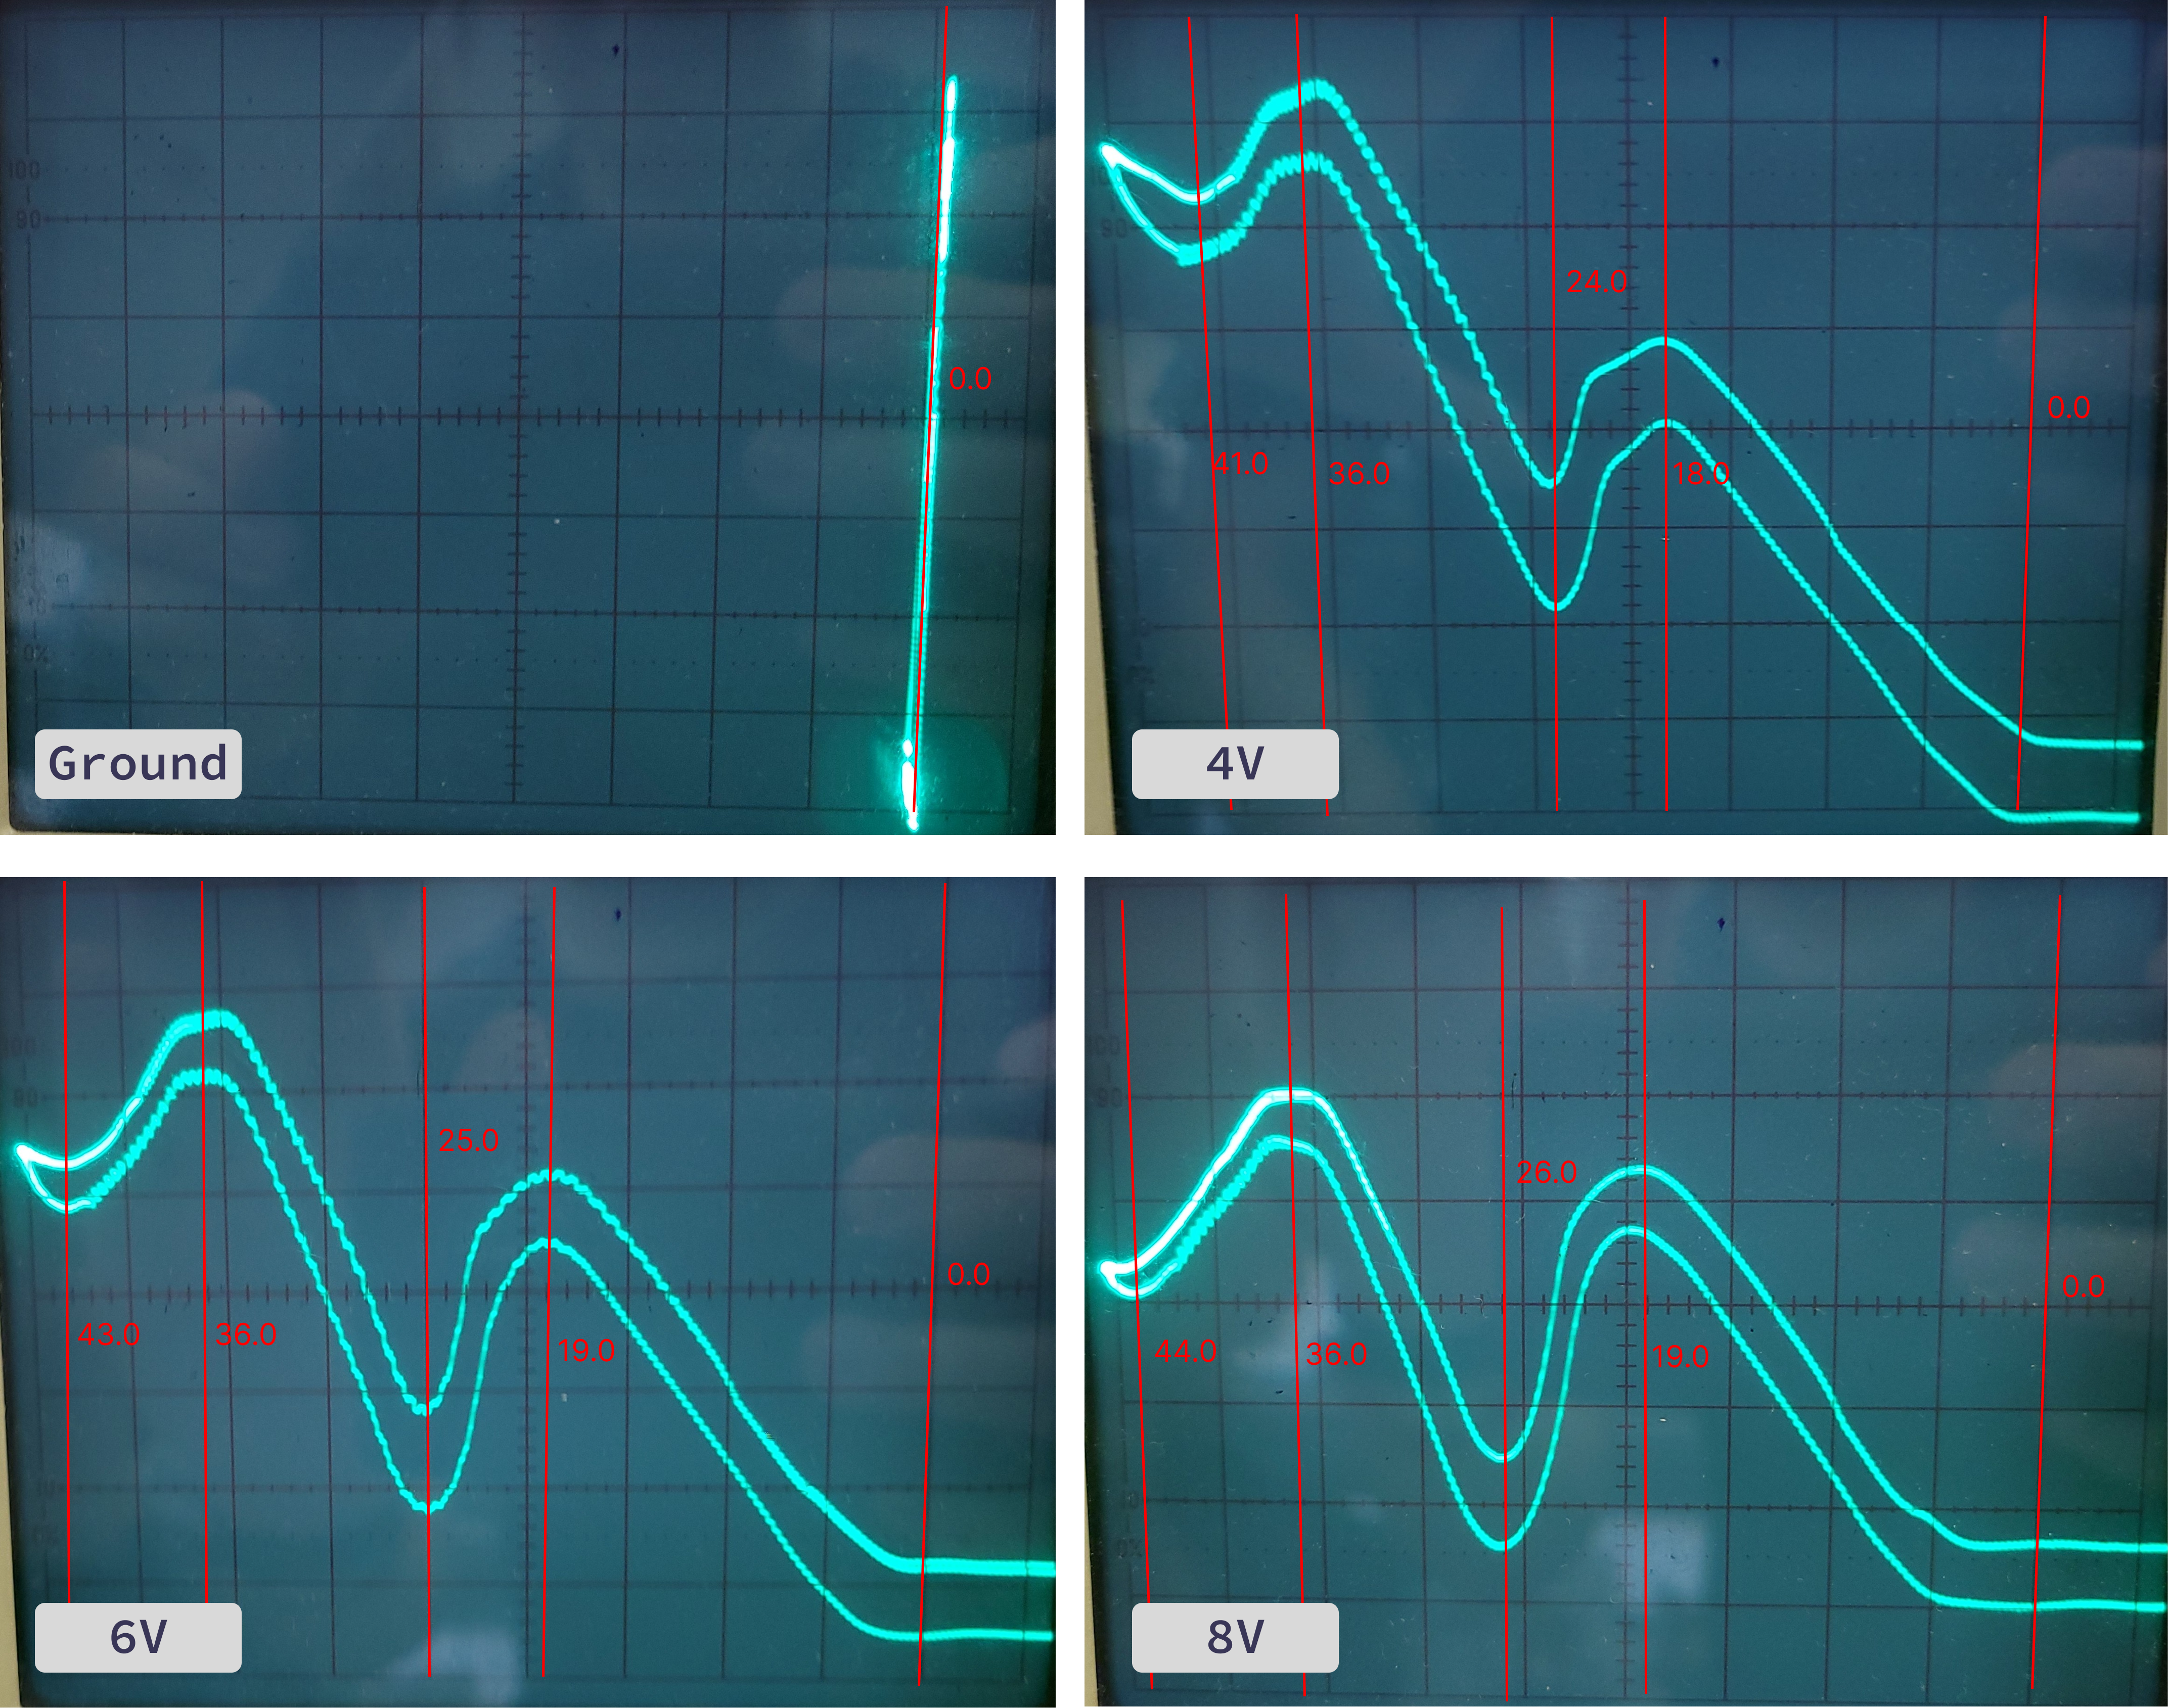
\includegraphics[width=0.8\linewidth]{photos/dyn.png}
		\caption{Зависимость тока коллектора от напряжения катод-.}
		\label{fig:dyn}
	\end{figure}
	
	\begin{table}[H]
		\footnotesize
		\begin{tabular}{lllll}
			\hline
			$V_{\text{разгон}}$, В & $V_{max}$, В   & $V_{min}$, В   & $V_{max}$, В   & $V_{min}$, В   \\ \hline
			4                      & $18.0 \pm 0.5$ & $24.0 \pm 1.0$ & $36.0 \pm 1.0$ & $41.0 \pm 1.0$ \\
			6                      & $19.0 \pm 0.5$ & $25.0 \pm 0.5$ & $36.0 \pm 1.0$ & $43.0 \pm 1.0$ \\
			8                      & $19.0 \pm 1.0$ & $26.0 \pm 0.5$ & $36.0 \pm 1.0$ & $44.0 \pm 1.0$ \\ \hline
		\end{tabular}
		\caption{Данные зависимости анодного тока от напряжения катод-сетка.}
		\label{tab:dyn}
	\end{table}
	
	Из осциллограм рассчитывая по максимумам получим: $\Delta V = (18.3 \pm 0.5)$ В.

	\newpage
	\subsection*{Статика}
	
	Измерения проводятся при трех значениях запирающего напряжения $V$.
	
	\begin{table}[H]
		\scriptsize
		\input{gen/data.tex}
		\caption{Данные зависимости коллекторного тока от напряжения катод-анод.}
		\label{tab:data}
	\end{table}
	
	\begin{figure}[H]
		\centering
		\includegraphics[width=0.8\linewidth]{gen/static.pdf}
		\caption{Зависимость коллекторного тока от разгоняющего напряжения.}
		\label{fig:static}
	\end{figure}
	
	Исходя из положений первых и вторых минимумов получим:
	\begin{equation}
		\Delta V = (19.3 \pm 0.4) \text{ В}
	\end{equation}
	
	Согласно справочным данным энергия перехода между основным и первым возбужденным состоянием составляет $\Delta V_{ref} = (19.8 \pm 0.1)$ В.
	
	Отметим, что данные, полученные динамическим методом, не находятся в пределах погрешности измерений. Предположительно, из-за инерционных эффектов первого метода, вносящих сильную ошибку измерений, поскольку на осциллограммах наблюдается различие ширины пиков прямого и обратного хода луча.

	\section*{Заключение и выводы}
	
	Работа подтверждает воспроизводимость результатов опыта Франка-Герца.
	
	В работе получено значение энергии перехода между основным и первым возбужденным состоянием атома гелия: $\Delta V = (19.3 \pm 0.4)$ В, в пределах погрешности совпадающее со справочным $\Delta V_{ref} = (19.8 \pm 0.1)$ В. 
\end{document}
